%\documentclass[cp, manuscript]{copernicus}
\documentclass[cp]{copernicus}

% Advances in Geosciences (adgeo)
% Advances in Radio Science (ars)
% Advances in Science and Research (asr)
% Advances in Statistical Climatology, Meteorology and Oceanography (ascmo)
% Annales Geophysicae (angeo)
% Atmospheric Chemistry and Physics (acp)
% Atmospheric Measurement Techniques (amt)
% Biogeosciences (bg)
% Climate of the Past (cp)
% Earth Surface Dynamics (esurf)
% Earth System Dynamics (esd)
% Earth System Science Data (essd)
% E&G Quaternary Science Journal (egqsj)
% Geoscientific Instrumentation, Methods and Data Systems (gi)
% Geoscientific Model Development (gmd)
% Hydrology and Earth System Sciences (hess)
% Journal of Sensors and Sensor Systems (jsss)
% Natural Hazards and Earth System Sciences (nhess)
% Nonlinear Processes in Geophysics (npg)
% Proceedings of the International Association of Hydrological Sciences (piahs)
% Scientific Drilling (sd)
% Solid Earth (se)
% The Cryosphere (tc)


%% \usepackage commands included in the copernicus.cls:
%\usepackage[german, english]{babel}
%\usepackage{tabularx}
%\usepackage{cancel}
%\usepackage{multirow}
%\usepackage{supertabular}
%\usepackage{algorithmic}
%\usepackage{algorithm}
%\usepackage{amsthm}
%\usepackage{float}
%\usepackage{subfig}
%\usepackage{rotating}
\usepackage{amsmath,amsfonts,amssymb}
\usepackage{url,hyperref}

\begin{document}
\title{Borehole Temperature Inversions: Information Content and Sensitivity}

\Author[1,2]{Volker}{Rath}
\Author[3]{Esther}{Heckenbach}
\Author[4]{Darius}{Mottaghy}
% \Author[5]{Ben}{Norden}
% \Author[6]{Sven}{Fuchs}

\affil[1]{Dublin Institute for Advanced Studies, Dublin, Ireland }
\affil[2]{Universit\'e de Savoie Montblanc, ISTerre, Le Bourget du Lac, France}
\affil[3]{Geoforschungszentrum, Potsdam, Germany}
\affil[4]{Aachen University of Applied Sciences, J\"ulich, Germany}
% \affil[5]{Geoforschungszentrum, Potsdam, Germany}
% \affil[6]{Geoforschungszentrum, Potsdam, Germany}



\runningtitle{Borehole inversions}

\runningauthor{Rath et al.}

\correspondence{Volker Rath (vrath@cp.dias.ie)}



\received{}
\pubdiscuss{} %% only important for two-stage journals
\revised{}
\accepted{}
\published{}

%% These dates will be inserted by Copernicus Publications during the typesetting process.


\firstpage{1}

\maketitle



\begin{abstract}
TEXT
\end{abstract}


\copyrightstatement{TEXT}


\introduction 
\label{sec:intro}
Recent measurements of borehole temperature profiles (BTPs) can be used to estimate past climate 
change from the ground surface temperature (GST). This is possible, because changes of surface 
temperatures diffuse into the sub­surface according to their period. While signals of 
high-frequency, like the annual temperature wave only pene­trate to a depth of 20~m, we can find 
the 
maximum signature of the last glacial maximum (LGM, $\approx$20~kyr BP) depths between 1000~m and 
2000~m, depending on the effective thermal diffusivity of the subsurface. A general de­scription of 
this method can be found in the monograph of \citet{Bodri2007a}. Since the seminal publi­cation of 
\citet{Lachenbruch1986a} this method has been employed in many studies on global, regional, or 
local 
scale (see the recent review of \citet{Gonzalez-Rouco2009a}, and the numerous references given 
therein). Most of these studies were based on very shallow boreholes (<500~m), thus only allowing a 
characterization of at most the last few centuries. Though already one of the first studies already 
dealt with the signature of the last glacial cycle \citep{Hotchkiss1934a}, the analysis of deeper 
boreholes has been less common 
\citep{Demezhko2014a, Kukkonen2011a, Kukkonen2011b, Chouinard2009a, Majorowicz2008a, Rath2007a,
Mottaghy2006a, Demezhko2001a, Clauser1995a}. This is partly because of the lack of appropriate 
boreholes, partly 
as the diffusion-like behavior of heat conduction implies that the resolution of GSTH 
reconstructions decreases fast with age \cite[e.g.][]{Demezhko2001a}. We expect dominant signatures 
from the temperature increase from the LGM to the Holocene at depths $>$1000~m. Earlier 
contributions will be much less prominent, only determining the integral pre-LGM behavior. 

\citet{Rath2012a} have pointed out that the last glacial cycle influences BTPs even at shallow 
depths, where its effect amounts to an additional heat flow density, which does not invalidate most 
of the earlier studies using this data, though increasing error \citep{Beltrami2011a, Rath2012a}. 
For boreholes deeper than 500~m but not resolving the LGM ($>$1500~m), the effects will be clearly 
visible. Knowing the effects of the ling-term GSTH is not only crucial in the paleoclimate-related 
interpretation, but also will improve the significant bias in the estimate of ``geothermal'' 
background heat­ flow \cite[e.g.][]{Westaway2013a,Majorowicz2011a,Slagstad2009a}. 


\section{Physical and mathematical background}

The task of deriving meaningful estimates of past climate changes, in particular GSTHs, from recent 
borehole temperature profiles (BTP) is nontrivial, because the problem is strongly ill-posed in the 
nomenclature of \citet{Hadamard1923a}. In a mathematical sense, the solutions to this problem may 
not exist, they may be non-unique, and possibly inherently unstable. Detailed accounts of this 
concept, and the techniques necessary to solve this kind of problems can be found in 
\citep{Hansen1998a, Hansen2010a} or \citep{Aster2019a}. In practice, this implies that the observed 
data (in this case the temperature measurements) need to be combined with knowledge from other 
sources to render the problem tractable. For the boreholes studied here, this additional 
information 
(as far as they are not introduced as explicit parameters in the Bayesian sense) includes a set of 
measured petrophysical properties, assumptions on the forward model used for the simulations, and 
on 
the general character of the solutions. It follows directly, that in these studies, goodness-of-fit 
cannot be the single criterion for the quality of the solution. 

Most current software for the estimation of GSTHs from borehole temperature profiles is based on a 
one-dimensional, conduction-only forward model.



\subsection{Forward model}
\label{sec:fwd}
The results presented in this article are based on one-dimensional, conduction-only forward 
modelling. Thermal conduction in rocks is based on the theory given by \citet{Carslaw1959a} for 
the heat conduction equation 

\begin{equation}\label{eqn:1}
 {\left( {\rho c} \right)_e}\frac{{\partial T}}{{\partial t}} + \frac{\partial 
}{{\partial z}}\left[ {{\lambda _e}\frac{{\partial T}}{{\partial z}}} \right] - 
H = 0{\text{ }.}
\end{equation} 

In this equation, $H$ denotes the volumetric heat production (W m$^{-3}$), while the index $e$ 
marks 
effective properties, i.e. properties which describe a rock-fluid-gas multi-phase system. As in the 
cases studied here porosity is very low, all properties will represent bulk rock properties, and 
the 
$e$ index will be omitted in the following. The occurring physical parameters are the density 
$\rho$ 
(kg m$^{-3}$), heat capacity $c_p$ (J kg$^{-1}$ K$^{-1}$), and thermal conductivity $\lambda$ (W 
m$^{-1}$ K$^{-1}$). The volumetric heat capacity is defined as $C = \rho c_p$. 
% diffusivity $\mu$ (m$^2$/s) 
% \begin{equation}\label{eqn:2}
% \mu = \frac{\lambda}{\rho c_p} = \frac{\lambda}{C}
% \end{equation} 

In order to solve Equation \ref{eqn:1} we assume a time-dependent Dirichlet boundary condition 
\begin{equation}\label{eqn:3a} 
T(z_0,t)=T_{GS}(t)
\end{equation} 
\noindent at the surface ($z=0$), and a stationary Neumann condition
\begin{equation}\label{eqn:3b}
\frac{\partial T}{\partial z}(z_{max }) = - \frac{q_b}{\lambda_e}
\end{equation} 
\noindent at the base of the model domain. Here, $q_b$ is the basal heat flow density at the base 
 of the model, $z_{max}$. 
 
This forward problem is solved by numerical finite difference techniques \cite[e.g.,][] 
{Patankar1980a}, allowing for a flexible discretization in both, time and space. As shown in 
Figure~\ref{fig:FD}, temperatures in this finite difference (FD) scheme are associated to nodes 
located at the boundary of the cells. Thermal conductivity $\lambda$, density $\rho$, heat capacity 
$c_p$, and heat production $H$ are associated with cells, but the latter is interpolated to the 
nodes for computational convenience. Time stepping is achieved by a Backward Euler or 
Crank-Nicholson scheme, which is complemented by a fixed point iteration for resolving the 
nonlinearities in the coefficients discussed in Section~\ref{sec:design}.


\begin{figure}[htp]
 \centering
 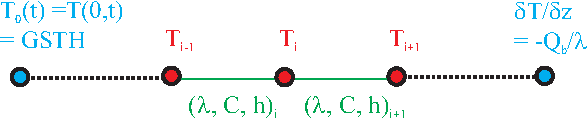
\includegraphics[width=\columnwidth]{Figures/FDScheme}
 \caption[Schematic description of the finite difference discretization.]{Schematic description of 
the discretization used for the finite difference forward modeling. Measured data have to be 
assigned to computational nodes (red), while the properties are associated with the cells. Both may 
imply interpolations or averaging (upscaling) to a given grid for observed temperatures and 
measured 
petrophysical properties.}
\label{fig:FD}
\end{figure}

\subsection{Inversion techniques}
\label{sec:tinv}
For the deterministic approach we seek to minimize an objective function $\Theta$ which is defined 
by

\begin{equation}\label{eqn:4}
\Theta = \mathcal{D}\left(\mathbf{d},\mathbf{m}\right) + \mathcal{R}\left(\mathbf{m} \right).
\end{equation} 
\noindent Here, the first term $\mathcal{D}$ measures the data fit, while the second, 
$\mathcal{R}$, 
is necessary to stabilize the generally ill-posed inverse problem, \cite[see][]{Aster2019a}. 

In this study, $\mathcal{D}$ is formulated as
\begin{equation} 
\mathcal{D} = 
 \left(\mathbf{d} - \mathbf{g(m)}\right)^T \mathbf{W}_d^T 
 \mathbf{W}_d^{}\left(\mathbf{d} - \mathbf{g(m)} \right)\quad,
\end{equation} 
\noindent where $\mathbf{W}_d$ denotes a weighting matrix commonly used to define the weighted 
residuals 
\begin{equation*}
\tilde{ \mathbf{r}} =\mathbf{W}_d^{}\mathbf{r} = 
\mathbf{W}_d^{} \left(\mathbf{d}-\mathbf{g}(\mathbf{m})\right)\quad, 
\end{equation*}
\noindent i.e., $\mathbf{W}_d = \mathbf{C}_d^{-1/2}$ is set to the inverse square root of the data 
covariance matrix $\mathbf{C}_d$, which assumed diagonal is in this study. 

In the problem treated here, the parameter vector $\mathbf{m}$ is composed of a piecewise constant 
function of time, using a logarithmic spacing. The data vector $\mathbf{d} = H(\mathbf{d}_{obs})$ 
contains the result of an observation operator $H$ applied to the discrete values of temperature 
measured in in the borehole. In this case, the application of this operator refers to the 
“upscaling” procedures mentioned in Section~\ref{sec:design}. This regularization in 
Equation~\ref{eqn:4} can be achieved in many different ways. Most of the results presented here use 
a generalized Tikhonov technique, formulating the corresponding term as

\begin{equation}
\label{eqn:5}
\begin{gathered}
 \mathcal{R}\left( {{\mathbf{m}} - {{\mathbf{m}}_a}} \right) = \hfill \\
 {\text{ }}\sum\nolimits_k {{\tau _k}} {\left( {{\mathbf{m}} - {{\mathbf{m}}_a}} 
\right)^T}{\mathbf{W}}_k^T{\mathbf{W}}_k^{}\left( {{\mathbf{m}} - {{\mathbf{m}}_a}} \right) \quad. 
\hfill \\ 
\end{gathered} 
\end{equation} 

In this equation, we define $\mathbf{W}_k$ to be a discrete approximation to the first derivative 
of 
the parameters with respect to logarithmic time, \cite[see][]{Aster2019a}, which can be written 
in discrete form using a logarithmic time step $h$:
 	 
\begin{equation}\label{eqn:6}
{{\mathbf{W}}_1} = \frac{1}{h}\left[ {\begin{array}{*{20}{c}}
 { - 1}&1&{}& \cdots &{}&0 \\ 
 {}&{ - 1}&1&{}&{}&{} \\ 
 \vdots &{}& \ddots &{}&{}& \vdots \\ 
 {}&{}&{}&{ - 1}&1&{} \\ 
 0&{}& \cdots &{}&{ - 1}&1 
\end{array}} \right]\end{equation} 

Taking the derivative of Equation~\ref{eqn:4}, and imposing the appropriate minimum conditions 
leads 
to the iteration
	
\begin{equation}\label{eqn:7}
\begin{gathered}
 \left(\mathbf{J}_w^T\mathbf{J}_w^{} + 
 \sum\limits_{i = 0}^1 \tau_i \mathbf{W}_{m,i}^T\mathbf{W}_{m,i}^{}\right) 
 \delta\mathbf{m}_k = \hfill \\
 \quad \quad \quad \quad \mathbf{J}_w^T\left[\mathbf{d}-
 \mathbf{g}(\mathbf{m}_k) \right] - \\
 \quad \quad \quad \quad \sum\limits_{i = 0}^1 \tau _i \mathbf{W}_{m,i} 
 \mathbf{W}_{m,i}^{}(\mathbf{m}_k - \mathbf{m}_a) \hfill \\ 
\end{gathered}
\end{equation} 

 \noindent with a subsequent update of the parameter vector by $\mathbf{m}_{k + 1} = \mathbf{m}_k + 
\mu \delta\mathbf{m}_k$.

We define the weighted Jacobian or sensitivity matrix as

\begin{equation}\label{eqn:8}
\mathbf{J}_w \equiv \mathbf{W}_d\mathbf{J} = 
\mathbf{W}_d\partial{\mathbf{g}}/\partial {\mathbf{m}}\quad, 
\end{equation} 

and the Generalized Inverse as

\begin{equation}\label{eqn:9}
\mathbf{J}_w^G = \left(\mathbf{J}_w^T \mathbf{J}_w^{} + 
\sum\limits_{i = 0}^1 \tau_i \mathbf{W}_{m,i}^T \mathbf{W}_{m,i}^{}\right)^{-1} 
\mathbf{J}_w^T{\text{ ,}}
\end{equation} 

respectively. Note that the inverse in Equation \ref{eqn:9} is the posterior covariance matrix. 
These quantities are appropriate tools to further analyze the sensitivity of given data to the 
inverse parameters. 

Given the two regularization parameters $\tau_0$ and $\tau_1$, this formulation can be seen an 
approximation to an inverse spatial exponential covariance a logarithmic scale with given error and 
correlation length \citep{Rodgers2000a, Tarantola2005a} For the inversions shown below, $\tau_0$ is 
set to a fixed small value (0.003), while $\tau_1$, is set to an optimal value determined by 
Generalized Cross Validation (GCV) \citep{Rath2007a,Farquharson2004a,Wahba1990a}. This optimal 
value 
is found by minimizing the GCV function 
\begin{equation}\label{eqn:10}
GCV(\tau ) = \frac
{N\left\| \mathbf{d} - \mathbf{g}(\mathbf{m}_\tau ^k) \right\|_2^2}
{\text{trace}
\left(\mathbf{I} - \mathbf{J}_w^{}\mathbf{J}_w^G \right)^2} 
\end{equation} 
\noindent over a set of predefined values of the regularization parameters $\tau$. For the 
inversions presented here, we always used the GCV criterion. The Unbiased Predictive Risk Estimator 
(UPRE) criterion described in \citet{Vogel2002a} produced nearly identical results. We did not use 
the L-curve approach described above, as this technique is not well adapted to non-linear inverse 
problems, where the identification of the point of maximal curvature often leads to highly 
improbable results. 

A useful measure for comparing the goodness-of-fit for different models is the normalized root mean 
square deviation (nRMS) defined by
 
\begin{equation}\label{eqn:11}
nRMS = \sqrt {\left( {{N_d} - 1} \right)_{}^{ - 1}\sum\nolimits_{j = 1}^N 
{{{\left( {\frac{{T_j^{obs}--T_j^{cal}}}{{{\sigma _j}}}} \right)}^2}} } \quad ,
\end{equation} 

where $N_d$ is the number of observations, and the second term under the root is the sum of 
standardized residuals. In the case of $N_d$ being large, and approximately Gaussian and independent 
data, the value should be near one. However, due to the many assumptions involved, small 
differences in nRMS are not considered as significant, and this parameter should only be used as an 
indicator. In particular, all runs shown here were run with a uniform error of 0.05~K for the 
temperature, which is usually a reasonable estimate for this quantity. Note that this error includes 
not only the measurement error, which is at least one order of magnitude smaller, but also some of 
errors related to an erroneous specification of the model (e.g., the use of average properties or 
interpolation). 

In contrast to the deterministic approach described above, which aim at deriving a single optimum 
model (often not catching the characteristics of all models compatible with the data), the Bayesian 
paradigm \cite[see, e.g.][] {Gelman2013a} aims not at a single GSTH which is optimal in a previously 
defined sense, but seeks to estimate the full posterior probability density function (PDF), given 
the prior PDF and the observational data. Detailed accounts on this approach can be found in 
\citep{Mosegaard1995a, Mosegaard2002a, Tarantola2005a}. This approach was used in 
\cite[][amongst others]{Kukkonen2011a, Kukkonen2011b, Kukkonen2015a, Rath2019a}. 
% 
% Deterministic inversions aim at deriving a single optimum model, which will commonly not catch the 
% characteristics of all models compatible with the data. In contrast, the stochastic methods 
% described in this section introduce constraints in generating a large number of models from a 
% random 
% set of temporally correlated models, as described below. Starting from the prior distribution by 
% $p(m)$ , and the conditional probability distribution, $p (d|m)$, also called likelihood, which 
% describes the probability that the data, $d$, will be observed, given a set of parameters $m$. 
% Given the above prior, we then seek the conditional (posterior) distribution of the model 
% parameter(s) given the data. We will denote this posterior probability distribution for the model 
% parameters by $p(m|d)$. Bayes’ theorem relates prior and posterior distributions by
%  
% \begin{equation}\label{eqn:12}
% p\left( {{\mathbf{m}}\left| {\mathbf{d}} \right.} \right) \propto p\left( 
% {{\mathbf{d}}\left| {\mathbf{m}} \right.} \right)p\left( {\mathbf{m}} \right)
% \end{equation} 
% 
% where the proportionality constant usually is not explicitly computed. While it is well known that, 
% under the restrictive assumption of Gaussian probabilities, estimators can be derived, which bear 
% some similarity to the deterministic methods described above \citep{Tarantola1982a,Tarantola1982b}, 
% the technique of choice for the Bayesian is of stochastic nature. In this study, a Markov Chain 
% Monte Carlo (MCMC) technique was employed. We used a variant of the well-known Metropolis-Hastings 
% algorithm (MH) \citep{Metropolis1953a, Hastings1970a,Haario2006a}. The Delayed Rejection Adaptive 
% Monte Carlo (DRAM) algorithm improves on MH, i) because it samples the posterior more effectively, 
% as the rejection of low-likelihood samples is delayed for a predefined number of steps in the MC 
% chain, before possibly being finally excludes, and ii) because it allows for an adaption of the 
% prior covariance during the progress of the MC chain. We used the DRAM algorithm as implemented by 
% \citet{Haario2006a}, with reduced or deactivated adaptivity in order to prevent a premature 
% concentration of models. There are problems with this choice in the case of an ill-posed inverse 
% problem as the one investigated here. The meaningfulness of the results depends strongly on the 
% reasonable choice of both prior probability density, which was chosen to be a multidimensional 
% Gaussian distribution $\mathcal{N}(mathbf{\mu},\mathbf{S})$. 
% 
% In DRAM, a predefined covariance 
% matrix $\mathbf{C}$ is updated at given intervals during the MC process. In our case, we did not 
% assume $\mathbf{C}$ to be diagonal, but allowed for temporal correlations in the GSTH parameters, 
% while for the remaining parameters ($Q_b$ and $H$) it was initialised with the appropriate 
% variances. For the parameters representing the GSTH, we introduced a Gaussian temporal covariance 
% matrix defined as
% 
% 
%  	f% Its width is controlled by a temporal correlation length $L$ of approximately half ofdecade, 
% which agrees with the resolution obtainable in this type of reconstruction \cite[e.g.,][] 
% {Demezhko2001a}. A number of chains were started in parallel, each starting from a perturbed 
% version of the prior which was set to the average of a GSTH derived from a Tikhonov deterministic 
% inversion 
% of the data set.

\section{Design of the numerical experiments}
\label{sec:design}

The general idea for the numerical experiments presented here is the following:

We have chosen a very simple homogeneous model, with two idealized GST histories. The first 
(``A'')is s simple step function at 10~ka BP, the second (``B'') is a slightly more complicated 
model taken from \cite{Balling1981a}. In order to avoid an ``inverse crime'' 
\cite[see][]{Kaipio2005a}, these models were simulated with a numerical code developed independently 
by \citet{Heckenbach2019a}.

In order to obtain a certain degree of realism in the synthetic BTPs, we chose to add noise to the 
simulations. We did not only add normally distributed noise, but imposed spatial correlations on 
the error series. For this purpose, we imposed an analytically defined exponential covariance on the 
noise, employing the well-known technique based on the Cholesky decomposition of the noise 
covariance matrix $\mathbf{C}_{n}=\mathbf{L}^T\mathbf{L}$, producing the correlated measurements 
by first generating normally distributed data $\mathbf{u}=\mathcal{N}(0,1)$, and then adding 
$\sigma_n = \mathbf{L}\mathbf{u}$ to the synthetic profiles. The covariance assumed for the  the 
simulation was the Gaussian, 
\begin{equation}\label{eqn:covg}
C_{i,j}^{{\text{gauss}}} = \sigma _i^2\exp \left[ {\frac{{ - {{\left| {{t_i} - 
{t_j}} \right|}^2}}}{{2{L^2}}}} \right] \quad , 
\end{equation}  
\noindent but could easily be replaced by an Markovian (exponential), or Mat\'ern matrix. The error 
amplitude amplitude is given by $\sigma_i$, while its width is controlled by a spatial
correlation length $L$. Both are varied in the numerical experiment in Section~\ref{sec:errors}. A 
similar procedure was employed for the perturbations of rock properties in Section~\ref{sec:props}.



Data and other relevant information site have to be pre-processed in a way appropriate for the 
given 
site, and assumptions have to be made accordingly. 

\subsection{Generation of Synthetic Borehole Temperature Profiles}

\section{Results}
\subsection{Numerical Experiment 1: Borehole temperature errors}\label{sec:errors}
\subsection{Numerical Experiment 2: Borehole length}\label{sec:length}
\subsection{Numerical Experiment 3: Basal heat flux}\label{sec:qb}
\subsection{Numerical Experiment 4: Rock Properties}\label{sec:props}


\conclusions %% \conclusions[modified heading if necessary]
Don't believe in Borehole Climatology!
%\appendix

\codedataavailability{The code for the generation and inversion relevant to this paper can be found 
at the \texttt{git} repository at \url{https:github.com/volkerrath/BTIsens.git}} 


\authorcontribution{
VR, DM, and EH developed the methodology and wrote the MATLAB codes used in this study. EH and VR 
designed and carried out the numerical simulations shown here. All authors took active part in the 
discussion of the results and writing the manuscript. 
} 

\competinginterests{
The authors declare that the research was conducted in the absence of any commercial or financial 
relationships that could represent a potential conflict of interest.
} 


\begin{acknowledgements}
We are grateful to Heikki Haario, Markko Laine, and Aslak Grinsted for making their MCMC software 
available. 
\end{acknowledgements}




%% REFERENCES

%% The reference list is compiled as follows:

\bibliographystyle{copernicus} 
\bibliography{RHetal2019}
%% Since the Copernicus LaTeX package includes the BibTeX style file copernicus.bst,
%% authors experienced with BibTeX only have to include the following two lines:
%%
%% \bibliographystyle{copernicus}
%% \bibliography{example.bib}
%%
%% URLs and DOIs can be entered in your BibTeX file as:
%%
%% URL = {http://www.xyz.org/~jones/idx_g.htm}
%% DOI = {10.5194/xyz}


%% LITERATURE CITATIONS
%%
%% command & example result
%% \citet{jones90}| & Jones et al. (1990)
%% \citep{jones90}| & (Jones et al., 1990)
%% \citep{jones90,jones93}| & (Jones et al., 1990, 1993)
%% \citep[p.~32]{jones90}| & (Jones et al., 1990, p.~32)
%% \citep[e.g.,][]{jones90}| & (e.g., Jones et al., 1990)
%% \citep[e.g.,][p.~32]{jones90}| & (e.g., Jones et al., 1990, p.~32)
%% \citeauthor{jones90}| & Jones et al.
%% \citeyear{jones90}| & 1990



%% FIGURES

%% When figures and tables are placed at the end of the MS (article in one-column style), please add \clearpage
%% between bibliography and first table and/or figure as well as between each table and/or figure.


%% ONE-COLUMN FIGURES

%%f
%\begin{figure}[t]
%\includegraphics[width=8.3cm]{FILE NAME}
%\caption{TEXT}
%\end{figure}
%
%%% TWO-COLUMN FIGURES
%
%%f
%\begin{figure*}[t]
%\includegraphics[width=12cm]{FILE NAME}
%\caption{TEXT}
%\end{figure*}
%
%
%%% TABLES
%%%
%%% The different columns must be seperated with a & command and should
%%% end with \\ to identify the column brake.
%
%%% ONE-COLUMN TABLE
%
%%t
%\begin{table}[t]
%\caption{TEXT}
%\begin{tabular}{column = lcr}
%\tophline
%
%\middlehline
%
%\bottomhline
%\end{tabular}
%\belowtable{} % Table Footnotes
%\end{table}
%
%%% TWO-COLUMN TABLE
%
%%t
%\begin{table*}[t]
%\caption{TEXT}
%\begin{tabular}{column = lcr}
%\tophline
%
%\middlehline
%
%\bottomhline
%\end{tabular}
%\belowtable{} % Table Footnotes
%\end{table*}
%
%%% LANDSCAPE TABLE
%
%%t
%\begin{sidewaystable*}[t]
%\caption{TEXT}
%\begin{tabular}{column = lcr}
%\tophline
%
%\middlehline
%
%\bottomhline
%\end{tabular}
%\belowtable{} % Table Footnotes
%\end{sidewaystable*}
%
%
%%% MATHEMATICAL EXPRESSIONS
%
%%% All papers typeset by Copernicus Publications follow the math typesetting regulations
%%% given by the IUPAC Green Book (IUPAC: Quantities, Units and Symbols in Physical Chemistry,
%%% 2nd Edn., Blackwell Science, available at: http://old.iupac.org/publications/books/gbook/green_book_2ed.pdf, 1993).
%%%
%%% Physical quantities/variables are typeset in italic font (t for time, T for Temperature)
%%% Indices which are not defined are typeset in italic font (x, y, z, a, b, c)
%%% Items/objects which are defined are typeset in roman font (Car A, Car B)
%%% Descriptions/specifications which are defined by itself are typeset in roman font (abs, rel, ref, tot, net, ice)
%%% Abbreviations from 2 letters are typeset in roman font (RH, LAI)
%%% Vectors are identified in bold italic font using \vec{x}
%%% Matrices are identified in bold roman font
%%% Multiplication signs are typeset using the LaTeX commands \times (for vector products, grids, and exponential notations) or \cdot
%%% The character * should not be applied as mutliplication sign
%
%
%%% EQUATIONS
%
%%% Single-row equation
%
%\begin{equation}
%
%\end{equation}
%
%%% Multiline equation
%
%\begin{align}
%& 3 + 5 = 8\\
%& 3 + 5 = 8\\
%& 3 + 5 = 8
%\end{align}
%
%
%%% MATRICES
%
%\begin{matrix}
%x & y & z\\
%x & y & z\\
%x & y & z\\
%\end{matrix}
%
%
%%% ALGORITHM
%
%\begin{algorithm}
%\caption{...}
%\label{a1}
%\begin{algorithmic}
%...
%\end{algorithmic}
%\end{algorithm}
%
%
%%% CHEMICAL FORMULAS AND REACTIONS
%
%%% For formulas embedded in the text, please use \chem{}
%
%%% The reaction environment creates labels including the letter R, i.e. (R1), (R2), etc.
%
%\begin{reaction}
%%% \rightarrow should be used for normal (one-way) chemical reactions
%%% \rightleftharpoons should be used for equilibria
%%% \leftrightarrow should be used for resonance structures
%\end{reaction}
%
%
%%% PHYSICAL UNITS
%%%
%%% Please use \unit{} and apply the exponential notation


\end{document}
